\subsection{Matrix Stats}\label{HiC:matrix-stats}% __08a-matrix-stats
%~~~~~~~~~~~~~~~~~~~%
\subsubsection{Input} % inputs
Data from the pipeline steps %\texttt{matrix-estimated}) (Section~\ref{HiC:matrix-estimated}), % this one removed
\texttt{matrix-filtered} (Section~\ref{HiC:matrix-filtered}), \texttt{matrix-hicnorm} (Section~\ref{HiC:matrix-hicnorm}), \texttt{matrix-prep} (Section~\ref{HiC:matrix-prep}), and \texttt{matrix-ic} (Section~\ref{HiC:matrix-ic}) are used as input.
%~~~~~~~~~~~~~~~~~~~%
\subsubsection{Analysis} % analysis
Default parameters:
\begin{lstlisting}
params.standard.tcsh$
#!/bin/tcsh

source ./inputs/params/params.tcsh

set chrom_excluded = 'chr[MY]'               # excluded chromosomes

\end{lstlisting}
%~~~~~~~~~~~~~~~~~~~%
\subsubsection{Output} % outputs
See Figure~\ref{fig:matrix-stats}. Default output: % results/matrix-stats.standard/matrix-filtered.by_sample.res_40kb/filter.by_sample.standard/align.by_sample.bowtie2/hg19/all-samples/
\begin{lstlisting}
-rw-r--r-- 1 at570  39K Feb 11 16:11 job.err
-rw-r--r-- 1 at570   47 Feb 11 15:48 job.id
-rw-r--r-- 1 at570    0 Feb 11 15:48 job.out
-rw-r--r-- 1 at570  480 Feb 11 15:48 job.sh
-rw-r--r-- 1 at570 5.3K Feb 11 16:11 job.vars.tsv
-rw-r--r-- 1 at570  59K Feb 11 16:11 stats.pdf
\end{lstlisting}

% ~/projects/hic-manual-report/report-base/figure/matrix-stats_stats.pdf
\begin{figure}[!htb]
    \centering
    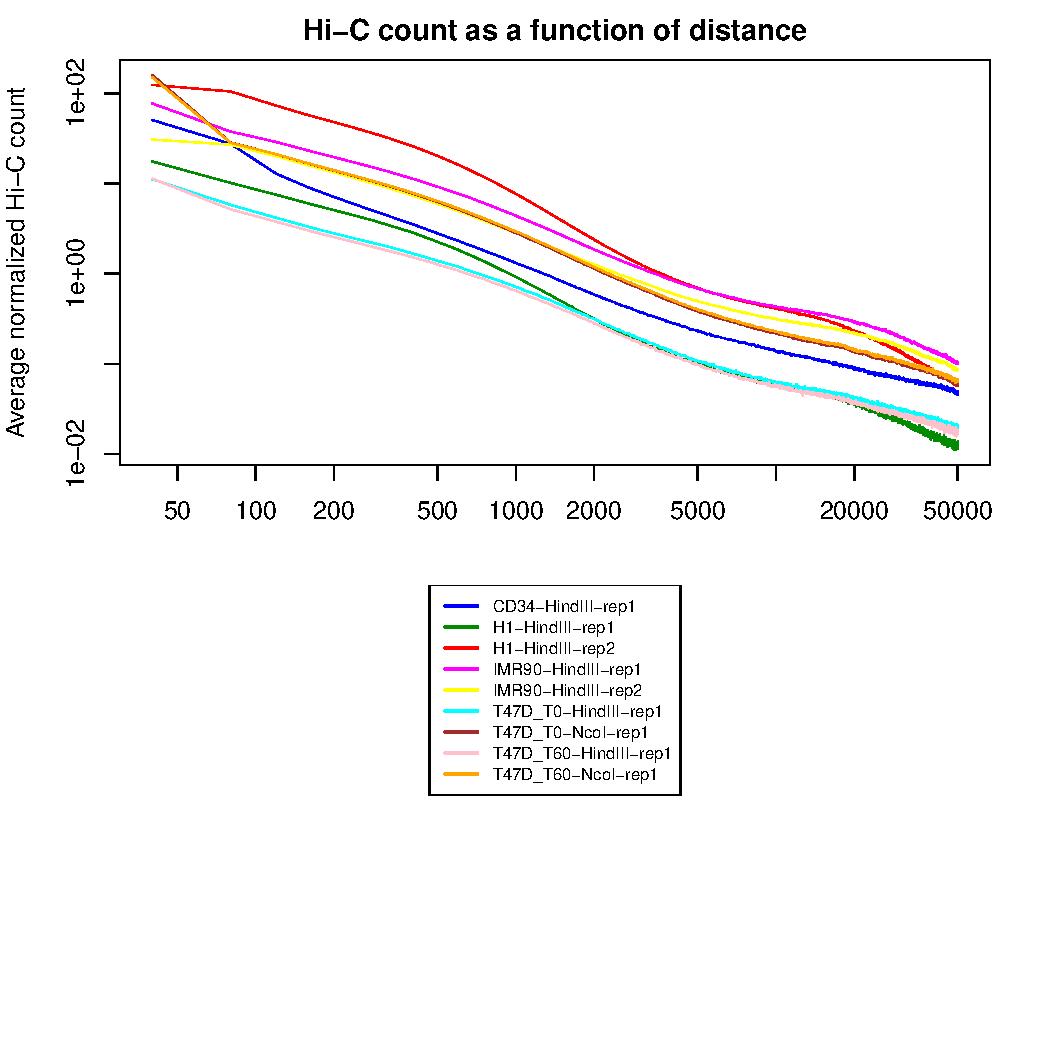
\includegraphics[width=\textwidth,height=\textheight,keepaspectratio]{figure/matrix-stats_stats}
    \caption{Matrix Stats sample output} % results/matrix-stats.standard/matrix-filtered.by_sample.res_40kb/filter.by_sample.standard/align.by_sample.bowtie2/hg19/all-samples/stats.pdf
    \label{fig:matrix-stats}
\end{figure}
% \newpage
\clearpage